% Declare type of document
\documentclass[10pt]{article}

% Import Packages
\usepackage[utf8]{inputenc} 

% Commonly used math symbols and fonts
\usepackage[mathscr]{euscript}
\usepackage{amsfonts,amsmath,amssymb,amsthm}
\usepackage{mathtools,mathdots}

% Better looking default font
\usepackage{lmodern}

% itemize environment
\usepackage{enumitem}
\usepackage{enumerate}

% Array, longtable, and booktabs
\usepackage{array}
\usepackage{longtable}
\usepackage{booktabs}
 
% Caption package for hiding Figure #
\usepackage{caption}

% Page formatting
\usepackage[letterpaper, margin=1in]{geometry}

% Package for nice syntax highlighting for code
% \usepackage[cache=false]{minted}
\usepackage{minted} 

% Allows line breaks in the math environment
\allowdisplaybreaks

\usepackage[activate={true,nocompatibility},final,tracking=true,kerning=true,spacing=true,factor=1100,stretch=10,shrink=10]{microtype}
\microtypecontext{spacing=nonfrench}
% activate={true,nocompatibility} - activate protrusion and expansion
% final - enable microtype; use "draft" to disable
% tracking=true, kerning=true, spacing=true - activate these techniques
% factor=1100 - add 10% to the protrusion amount (default is 1000)
% stretch=10, shrink=10 - reduce stretchability/shrinkability (default is 20/20)



\usepackage{multicol}




\title{CS 310: Hashing (Part I)}
\author{Connor Baker}
\date{February 26, 2019}

\begin{document}

\maketitle

\begin{center}
    \begin{tabular}{lcccccr} \toprule
        Implementation & get/set & add/del at end & add/del start & add/del mid & search & can grow? \\ \midrule
        Static Array & 1 & 1 & $N$ & $N$ & $N$ & no \\
        Dynamic Array & 1 & $\mathbf{1^*}$ & $N$ & $N$ & $N$ & no \\
        Singly-Linked & $N$ & 1, $N$ & 1 & $N$ & $N$ & yes \\
        Doubly-Linked & $N$ & 1 & 1 & $N$ & $N$ & yes \\ 
        Stack & 1 (top) & 1 (pop) & 1 (push) & - & - & yes \\
        Queue & 1 (getFront) & 1 (enqueue) & 1 (dequeue) & - & - & yes \\ \bottomrule
    \end{tabular}
    \begin{center}*Amortized analysis\end{center}
\end{center}

\subsection*{Motivation}
\begin{itemize}
    \item Task: suggest a data structure that can support retrieval and deletion of any value in constant time
    \begin{itemize}
        \item \mintinline{java}{.add(T t)}, \mintinline{java}{.remove(T t)}, and \mintinline{java}{.has(T t)} are $O(n)$
    \end{itemize}
    \item What should we do if the value we want to remove is in some range, $[a,b]$?
    \begin{itemize}
        \item An array would work best here, because we have a contiguous range
        \item Could use something like \mintinline{java}{myArray[b-a]} where \mintinline{java}{myArray[i-a]} indicates whether we have added an integer $i$ into our storage
        \begin{itemize}
            \item Initialize the entire array to zero to make it clear that it contains no elements
            \item How would we perform \mintinline{java}{.add(T t)}, \mintinline{java}{.remove(T t)}, or \mintinline{java}{.has(T t)}?
        \end{itemize}
    \end{itemize}
    \item So an array works to tell us if something is in the set, because we can use the value at each index as a true or false boolean that tells us whether we have the element at the index
    \item What we would like \textit{in general} is a mapping from any \mintinline{java}{Object} to some small manageable integer
    \begin{itemize}
        \item We call this mapping a \textit{hashing}
    \end{itemize}
\end{itemize}

\subsection*{Terminology}
\begin{itemize}
    \item \textit{Hash code}: the integer computer for any object
    \item \textit{Hash function}: the function that computes a hash code for any object
    \item \textit{Hash table}
    \begin{itemize}
        \item Storage of objects based on their hash codes
        \begin{itemize}
            \item Use a has code to perform a fast table lookup
        \end{itemize}
        \item Looks a lot like an array or a linked list
        \item Usually we do not keep duplicates -- duplicate elements get mapped to the same place in the hash table
    \end{itemize}
\end{itemize}

\subsection*{Hash Table Example}
\begin{center}
    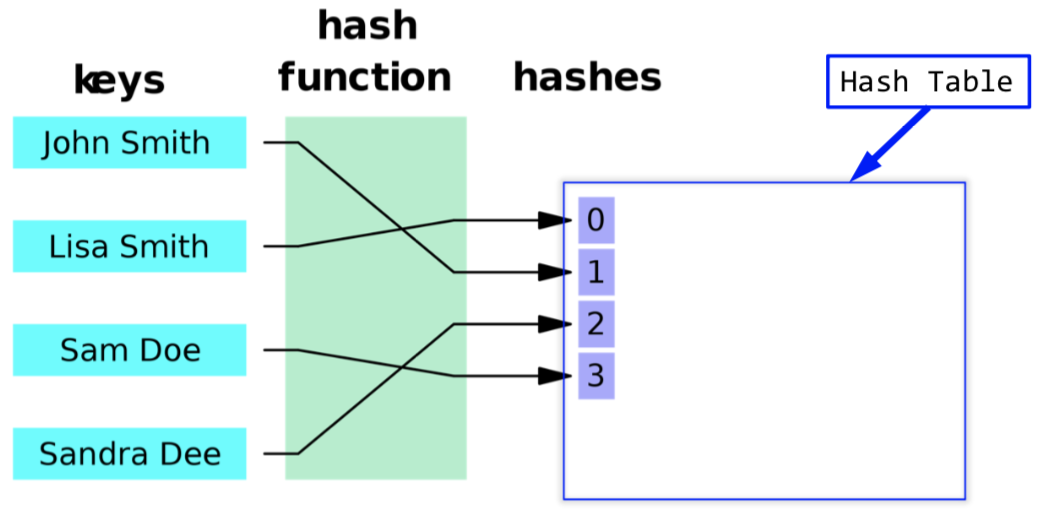
\includegraphics[width=0.5\linewidth]{images/1.png}    
\end{center}

\subsection*{Hash Table}
\begin{itemize}
    \item Store objects in an array in a retrievable way
    \item A simplified view of \mintinline{java}{.add(T t)}:
    \begin{itemize}
        \item Compute the integer hash code \mintinline{java}{xhc} from \mintinline{java}{x}
        \item Put \mintinline{java}{x} in an array \mintinline{java}{hta} at the index \mintinline{java}{xhc}
    \end{itemize}
    \item Things to consider
    \begin{itemize}
        \item How do you compute \mintinline{java}{xhc}? Where should that code exist?
        \item What if \mintinline{java}{xhc} is too big (it's larger than the length of the hash table)?
        \item What if the current index is occupied?
        \begin{itemize}
            \item We call this a \textit{hash collision}
        \end{itemize}
    \end{itemize}
\end{itemize}

\subsection*{Roadmap}
\begin{itemize}
    \item Basic ideas of hashing
    \item Hash code computation
    \item Using hash codes
    \begin{itemize}
        \item Bounding the range
        \item Hash table collision resolution and other strategies
    \end{itemize}
\end{itemize}

\subsection*{Hash Code}
\begin{itemize}
    \item An integer computed for an object
    \item Every object in Java has a \mintinline{java}{.hashCode()} method
    \begin{itemize}
        \item \mintinline{java}{int hc = thing.hashCode();}
        \item By default, \mintinline{java}{Object}'s \mintinline{java}{.hashCode()} is invoked (since all objects extend \mintinline{java}{Object}), which typically converts the memory address to an integer and uses that (though this behavior isn't required by the JVM)
        \item Official documentation
    \end{itemize}
\end{itemize}

\subsection*{Overriding \mintinline{java}{.hashCode()}}
\begin{itemize}
    \item We can override \mintinline{java}{.hashCode()} to do something special on a per-class basis
    \begin{itemize}
        \item For your own classes, override the default \mintinline{java}{.hashCode()}
        \item Compute the hash based on the internal data of an object
        \item Follow the hash contract
    \end{itemize}
    \begin{minted}{java}
    public class Student {
        Integer gnumber;
        String name;
        Department dept;

        // Other methods omitted

        @Override
        public int hashCode() { return gnumber.hashCode(); }
    }
    \end{minted}
\end{itemize}

\subsection*{Hash Contract}
\begin{itemize}
    \item \mintinline{java}{x.equals(y)} $\implies$ \mintinline{java}{x.hashCode() == y.hashCode()}
    \begin{itemize}
        \item However, \textit{different objects can have the same hash code}
    \end{itemize}
    \item We can revisit our code snippet from above and make the hash more resilient
    \begin{minted}{java}
public class Student {
    Integer gnumber;
    String name;
    Department dept;

    // Other methods omitted

    @Override
    public int hashCode() { return gnumber.hashCode() + dept.hashCode(); }
}
        \end{minted}
\end{itemize}

\subsection*{Picking a Good Hash Function}
\begin{itemize}
    \item Adhere to the \textit{Hash Contract}
    \begin{itemize}
        \item If $x = y$ then they must have the same hash
    \end{itemize}
    \item \textit{Distribute} different objects ``fairly'' across the integers
    \begin{itemize}
        \item We get reduced collision as a benefit of this
    \end{itemize}
    \item Compute the hash code as \textit{quickly} as possible
    \begin{itemize}
        \item Since we'll be doing a lot of hashing, we can greatly speed up the hash table with a fast hash function
    \end{itemize}
    \item \textit{Note}: We can't usually get all three of these, so we have to decide which, based on the problem, need to be prioritized 
\end{itemize}

\subsection*{Hash Table (a Simplified View)}
\begin{itemize}
    \item Store objects in an array \mintinline{java}{hta} in a retrievable way
    \item \mintinline{java}{.add(T t)}: put the object \mintinline{java}{t} in the hash table
    \begin{itemize}
        \item Compute the hash code \mintinline{java}{thc} from \mintinline{java}{t}
        \item Use \mintinline{java}{thc} as the index of \mintinline{java}{hta} in which we will store \mintinline{java}{t}
    \end{itemize}
    \item \mintinline{java}{.has(T t)}: check if \mintinline{java}{t} is in the hash table
    \begin{itemize}
        \item Compute the hash code \mintinline{java}{thc} from \mintinline{java}{t}
        \item \mintinline{java}{return t.equals(hta[thc]);}
    \end{itemize}
    \item \mintinline{java}{.remove(T t)}: delete \mintinline{java}{t} from the hash table
    \begin{itemize}
        \item Compute the hash code \mintinline{java}{thc} from \mintinline{java}{t}
        \item \mintinline{java}{if has(t) { hta[thc] = null;}}
    \end{itemize}
\end{itemize}


\subsection*{Hash Table: Issues}
\begin{minted}{java}
class HashSet<T> {
    T hta[];
    int size;

    void add(T x) {
        int xhc = x.hashCode();
        // What if xhc is out of bounds?
        // What if this entry is already occupied?
        hta[xhc] = x;
        size++;
    }

    boolean has(T x) {
        int xhc = x.hashCode();
        return x.equals(this.hta[xhc]);
    }
}
\end{minted}


\subsection*{Hash Code Processing}
\begin{itemize}
    \item Modulo (remainder) is the typical way to bound the hash code based on the hash table length:
    \begin{minted}{java}
int n = hta.length;
hta[abs(xhc) % n] = x;        
    \end{minted}
    \item For math-related reasons, it's usually best to make $n$ a larger \textit{prime} number
    \begin{itemize}
        \item We do this so that multiples of the same number modulo $n$ are less likely to collide
    \end{itemize}
    \begin{multicols}{2}
    \begin{itemize}
        \item[]\begin{minted}{java}
30 % 17 = 13
300 % 17 = 11
3000 % 17 = 8
30000 % 17 = 12
        \end{minted}
        \item[]\begin{minted}{java}
30 % 9 = 3
300 % 9 = 3
3000 % 9 = 3
30000 % 9 = 3
        \end{minted}
    \end{itemize}
    \end{multicols}
    \item Now we have bounding issues resolved, but we've shortened the range
    \begin{itemize}
        \item It's more likely now that we'll have different objects mapping to the same entry
    \end{itemize}
\end{itemize}

\subsection*{Hash Table Collisions}
\begin{itemize}
    \item Motivation
    \begin{itemize}
        \item Put \mintinline{java}{x} in a table at \mintinline{java}{hta[xhc]}
        \item \textbf{Problem}: what if \mintinline{java}{hta[xhc]} is occupied?
        \item \textbf{Answer}: find some other storage for \mintinline{java}{x}
    \end{itemize}
    \item Common approaches
    \begin{itemize}
        \item Separate chaining
        \item Open addressing
    \end{itemize}
\end{itemize}

\subsection*{Separate Chaining}
\begin{itemize}
    \item Something already there?
    \begin{itemize}
        \item Expand that single entry into an internal data structure
        \begin{itemize}
            \item This way we can accommodate multiple objects which have the same hash code
            \item We can also grow this structure if we get more collisions
        \end{itemize}
        \item We have a data structure for this... what is it?
        \begin{itemize}
            \item A linked list (or an array list)
        \end{itemize}
        \item \textbf{What's the worst case complexity?}
        \begin{itemize}
            \item \textbf{How can we avoid that case?}
        \end{itemize}
    \end{itemize}
\end{itemize}

\subsection*{Separate Chaining Examples}
\subsubsection*{Example 1}
\setlength\columnsep{15em}
\begin{multicols}{2}
\begin{itemize}
    \item[] \begin{minted}{java}
String [] sa1 = new String[] {
    "Chris",
    "Sam",
    "Beth",
    "Dan"
};
SeparateChainHS<String> h = new SeparateChainHS<String>(11);
for(String s : sa1) {
    h.add(s);
}
// String("Chris").hashCode() % 11=65087095 % 11 = 7
// String("Sam").hashCode() % 11=82879 % 11 = 5
// String("Beth").hashCode() % 11=68465 % 11 = 1
// String("Dan").hashCode() % 11=2066967 % 11 = 1
\end{minted}
\item[] 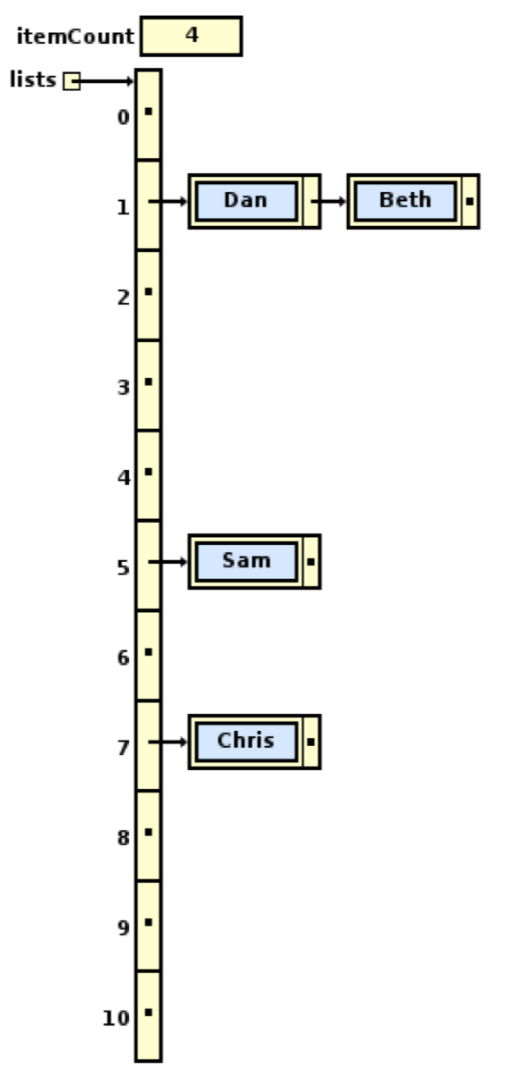
\includegraphics[width=0.26\textwidth]{images/2.png}
\end{itemize}
\end{multicols}
\begin{itemize}
    \item Every table entry is a linked list
    \begin{itemize}
        \item \mintinline{java}{hta[i]} stores all the values mapping to index \mintinline{java}{i}
    \end{itemize}
    \item Example:
    \begin{itemize}
        \item Table length = 11
        \item Number of items = 4
        \item Load: $$\frac{\text{item count}}{\text{hash table length}} = \frac{4}{11} \approx 0.\overline{36}$$
    \end{itemize}
\end{itemize}

\subsubsection*{Example 2}
\begin{multicols}{2}
\begin{itemize}
\item[]\begin{minipage}[t]{\linewidth}
\begin{itemize}
    \item Table length = 11
    \item Number of items = 4
    \item Load:
     $$\frac{\text{item count}}{\text{hash table length}} = \frac{14}{11}$$
     $$\frac{14}{11} = \approx 1.\overline{27}$$
\end{itemize}
\end{minipage}
\item[] 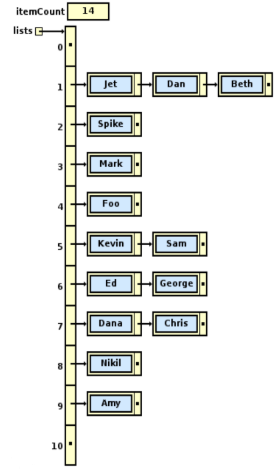
\includegraphics[width=0.3\textwidth]{images/3.png}
\end{itemize}
\end{multicols}

\subsubsection*{Discussion}
\begin{itemize}
    \item Why use an array of linked lists?
    \item How can we calculate a good load factor?
\end{itemize}


\subsection*{Separate Chaining Analysis}
\begin{itemize}
    \item \mintinline{java}{.add(T t)} is $O(1)$ assuming adding to a list is $O(1)$ and that duplicates are allowed
    \begin{itemize}
        \item If duplicates aren't allowed, the time jumps to $O(n)$ since we need to search the chain to make sure that we don't already have the element in the chain
    \end{itemize}
    \item \mintinline{java}{.remove(T t)}/\mintinline{java}{.contains(T t)}
    \begin{itemize}
        \item The run time depends on the number of things in each list
        \item \mintinline{java}{.remove(T t)}/\mintinline{java}{.contains(T t)} must potentially look through all elements in the longest chain in the hash table to see if \mintinline{java}{t} is present
        \begin{itemize}
            \item The average case is $O($average chain length$)= O($\mintinline{java}{itemCount/tableLength}$)=O($load$)$
            \item The worst case time is $O($\mintinline{java}{itemCount}$)$
            \item How do we avoid the worst case?
        \end{itemize}
    \end{itemize}
\end{itemize}

\subsection*{Separate Chaining is Viable in Practice}
\begin{itemize}
    \item It's relatively simple to implement (see Weiss Fig. 20.20)
    \item It's reasonably efficient
    \item Java's built-in hash tables use it
    \begin{itemize}
        \item \mintinline{java}{java.util.HashSet}, \mintinline{java}{java.util.HashMap}, and \mintinline{java}{java.util.Hashtable} all use separate chaining
    \end{itemize}
\end{itemize}

\end{document}